
\documentclass[a4paper,11pt]{article}
\usepackage[a4paper, margin=8em]{geometry}

% usa i pacchetti per la scrittura in italiano
\usepackage[french,italian]{babel}
\usepackage[T1]{fontenc}
\usepackage[utf8]{inputenc}
\frenchspacing 

% usa i pacchetti per la formattazione matematica
\usepackage{amsmath, amssymb, amsthm, amsfonts}

% usa altri pacchetti
\usepackage{gensymb}
\usepackage{hyperref}
\usepackage{standalone}

\usepackage{colortbl}

\usepackage{xstring}
\usepackage{karnaugh-map}

% imposta il titolo
\title{Electronics for Embedded Systems notes}
\author{Luca Seggiani}
\date{2026}

% spaziatura liste
\usepackage{enumitem}
\setlist[itemize]{noitemsep, topsep=4pt, partopsep=0pt, parsep=2pt, leftmargin=*}
\setlist[enumerate]{noitemsep, topsep=4pt, partopsep=0pt, parsep=2pt, leftmargin=*}

% imposta lo stile
% usa helvetica
\usepackage[scaled]{helvet}
% usa palatino
\usepackage{palatino}
% usa un font monospazio guardabile
\usepackage{lmodern}

\renewcommand{\rmdefault}{ppl}
\renewcommand{\sfdefault}{phv}
\renewcommand{\ttdefault}{lmtt}

% circuiti
\usepackage{circuitikz}
\usetikzlibrary{babel}

% testo cerchiato
\newcommand*\circled[1]{\tikz[baseline=(char.base)]{
            \node[shape=circle,draw,inner sep=2pt] (char) {#1};}}

% disponi il titolo
\makeatletter
\renewcommand{\maketitle} {
	\begin{center} 
		\begin{minipage}[t]{.8\textwidth}
			\textsf{\huge\bfseries \@title} 
		\end{minipage}%
		\begin{minipage}[t]{.2\textwidth}
			\raggedleft \vspace{-1.65em}
			\textsf{\small \@author} \vfill
			\textsf{\small \@date}
		\end{minipage}
		\par
	\end{center}

	\thispagestyle{empty}
	\pagestyle{fancy}
}
\makeatother

% disponi teoremi
\usepackage{tcolorbox}
\newtcolorbox[auto counter, number within=section]{theorem}[2][]{%
	colback=blue!10, 
	colframe=blue!40!black, 
	sharp corners=northwest,
	fonttitle=\sffamily\bfseries, 
	title=Theorem~\thetcbcounter: #2, 
	#1
}

% disponi definizioni
\newtcolorbox[auto counter, number within=section]{definition}[2][]{%
	colback=red!10,
	colframe=red!40!black,
	sharp corners=northwest,
	fonttitle=\sffamily\bfseries,
	title=Definition~\thetcbcounter: #2,
	#1
}

% disponi codice
\usepackage{listings}
\usepackage[table]{xcolor}

\definecolor{codegreen}{rgb}{0,0.6,0}
\definecolor{codegray}{rgb}{0.5,0.5,0.5}
\definecolor{codepurple}{rgb}{0.58,0,0.82}
\definecolor{backcolour}{rgb}{0.95,0.95,0.92}

\lstdefinestyle{codestyle}{
		backgroundcolor=\color{black!5}, 
		commentstyle=\color{codegreen},
		keywordstyle=\bfseries\color{magenta},
		numberstyle=\sffamily\tiny\color{black!60},
		stringstyle=\color{green!50!black},
		basicstyle=\ttfamily\footnotesize,
		breakatwhitespace=false,         
		breaklines=true,                 
		captionpos=b,                    
		keepspaces=true,                 
		numbers=left,                    
		numbersep=5pt,                  
		showspaces=false,                
		showstringspaces=false,
		showtabs=false,                  
		tabsize=2
}

\lstdefinestyle{shellstyle}{
		backgroundcolor=\color{black!5}, 
		basicstyle=\ttfamily\footnotesize\color{black}, 
		commentstyle=\color{black}, 
		keywordstyle=\color{black},
		numberstyle=\color{black!5},
		stringstyle=\color{black}, 
		showspaces=false,
		showstringspaces=false, 
		showtabs=false, 
		tabsize=2, 
		numbers=none, 
		breaklines=true
}

\lstdefinelanguage{x86}{ 
  keywords={AAA, AAD, AAM, AAS, ADC, ADCB, ADCW, ADCL, ADD, ADDB, ADDW, ADDL, AND, ANDB, ANDW, ANDL,
        ARPL, BOUND, BSF, BSFL, BSFW, BSR, BSRL, BSRW, BSWAP, BT, BTC, BTCB, BTCW, BTCL, BTR, 
        BTRB, BTRW, BTRL, BTS, BTSB, BTSW, BTSL, CALL, CBW, CDQ, CLC, CLD, CLI, CLTS, CMC, CMP,
        CMPB, CMPW, CMPL, CMPS, CMPSB, CMPSD, CMPSW, CMPXCHG, CMPXCHGB, CMPXCHGW, CMPXCHGL,
        CMPXCHG8B, CPUID, CWDE, DAA, DAS, DEC, DECB, DECW, DECL, DIV, DIVB, DIVW, DIVL, ENTER,
        HLT, IDIV, IDIVB, IDIVW, IDIVL, IMUL, IMULB, IMULW, IMULL, IN, INB, INW, INL, INC, INCB,
        INCW, INCL, INS, INSB, INSD, INSW, INT, INT3, INTO, INVD, INVLPG, IRET, IRETD, JA, JAE,
        JB, JBE, JC, JCXZ, JE, JECXZ, JG, JGE, JL, JLE, JMP, JNA, JNAE, JNB, JNBE, JNC, JNE, JNG,
        JNGE, JNL, JNLE, JNO, JNP, JNS, JNZ, JO, JP, JPE, JPO, JS, JZ, LAHF, LAR, LCALL, LDS,
        LEA, LEAVE, LES, LFS, LGDT, LGS, LIDT, LMSW, LOCK, LODSB, LODSD, LODSW, LOOP, LOOPE,
        LOOPNE, LSL, LSS, LTR, MOV, MOVB, MOVW, MOVL, MOVSB, MOVSD, MOVSW, MOVSX, MOVSXB,
        MOVSXW, MOVSXL, MOVZX, MOVZXB, MOVZXW, MOVZXL, MUL, MULB, MULW, MULL, NEG, NEGB, NEGW,
        NEGL, NOP, NOT, NOTB, NOTW, NOTL, OR, ORB, ORW, ORL, OUT, OUTB, OUTW, OUTL, OUTSB, OUTSD,
        OUTSW, POP, POPL, POPW, POPB, POPA, POPAD, POPF, POPFD, PUSH, PUSHL, PUSHW, PUSHB, PUSHA, 
        RCLL, RCR, RCRB, RCRW, RCRL, RDMSR, RDPMC, RDTSC, REP, REPE, REPNE, RET, ROL, ROLB, ROLW,
        ROLL, ROR, RORB, RORW, RORL, SAHF, SAL, SALB, SALW, SALL, SAR, SARB, SARW, SARL, SBB,
        SBBB, SBBW, SBBL, SCASB, SCASD, SCASW, SETA, SETAE, SETB, SETBE, SETC, SETE, SETG, SETGE,
        SETL, SETLE, SETNA, SETNAE, SETNB, SETNBE, SETNC, SETNE, SETNG, SETNGE, SETNL, SETNLE,
        SETNO, SETNP, SETNS, SETNZ, SETO, SETP, SETPE, SETPO, SETS, SETZ, SGDT, SHL, SHLB, SHLW,
        SHLL, SHLD, SHR, SHRB, SHRW, SHRL, SHRD, SIDT, SLDT, SMSW, STC, STD, STI, STOSB, STOSD,
        STOSW, STR, SUB, SUBB, SUBW, SUBL, TEST, TESTB, TESTW, TESTL, VERR, VERW, WAIT, WBINVD,
        XADD, XADDB, XADDW, XADDL, XCHG, XCHGB, XCHGW, XCHGL, XLAT, XLATB, XOR, XORB, XORW, XORL},
  keywordstyle=\color{blue}\bfseries,
  ndkeywordstyle=\color{darkgray}\bfseries,
  identifierstyle=\color{black},
  sensitive=false,
  comment=[l]{\#},
  morecomment=[s]{/*}{*/},
  commentstyle=\color{purple}\ttfamily,
  stringstyle=\color{red}\ttfamily,
  morestring=[b]',
  morestring=[b]"
}

\lstdefinelanguage{riscv}{
  keywords={
    LUI, AUIPC,
    JAL, JALR,
    BEQ, BNE, BLT, BGE, BLTU, BGEU,
    LB, LH, LW, LBU, LHU, LD,
    SB, SH, SW, SD,
    ADDI, SLTI, SLTIU, XORI, ORI, ANDI,
    SLLI, SRLI, SRAI,
    ADD, SUB, SLL, SLT, SLTU, XOR, SRL, SRA, OR, AND,
    ADDIW, SLLIW, SRLIW, SRAIW,
    ADDW, SUBW, SLLW, SRLW, SRAW,
    MUL, MULH, MULHSU, MULHU, DIV, DIVU, REM, REMU,
    MULW, DIVW, DIVUW, REMW, REMUW,
    LR.W, SC.W, AMOSWAP.W, AMOADD.W, AMOXOR.W,
    AMOAND.W, AMOOR.W, AMOMIN.W, AMOMAX.W,
    AMOMINU.W, AMOMAXU.W,
    LR.D, SC.D, AMOSWAP.D, AMOADD.D, AMOXOR.D,
    AMOAND.D, AMOOR.D, AMOMIN.D, AMOMAX.D,
    AMOMINU.D, AMOMAXU.D,
    FLW, FSW,
    FMADD.S, FMSUB.S, FNMSUB.S, FNMADD.S,
    FADD.S, FSUB.S, FMUL.S, FDIV.S, FSQRT.S,
    FSGNJ.S, FSGNJN.S, FSGNJX.S,
    FMIN.S, FMAX.S,
    FCVT.W.S, FCVT.WU.S, FCVT.S.W, FCVT.S.WU,
    FMV.X.W, FMV.W.X,
    FEQ.S, FLT.S, FLE.S,
    FLD, FSD,
    FMADD.D, FMSUB.D, FNMSUB.D, FNMADD.D,
    FADD.D, FSUB.D, FMUL.D, FDIV.D, FSQRT.D,
    FSGNJ.D, FSGNJN.D, FSGNJX.D,
    FMIN.D, FMAX.D,
    FCVT.W.D, FCVT.WU.D, FCVT.D.W, FCVT.D.WU,
    FCVT.S.D, FCVT.D.S,
    FMV.X.D, FMV.D.X,
    FEQ.D, FLT.D, FLE.D,
    CSRRW, CSRRS, CSRRC,
    CSRRWI, CSRRSI, CSRRCI,
    FENCE.I,
    FENCE,
    ECALL, EBREAK,
    MRET, SRET, URET,
    WFI,
    SFENCE.VMA,
    NOP, LI, LA, MV,
    NOT, NEG, NEGW,
    SEQZ, SNEZ, SLTZ, SGTZ,
    BEQZ, BNEZ, BLEZ, BGEZ, BLTZ, BGTZ,
    BGT, BLE, BGTU, BLEU,
    J, JR, RET,
    CALL, TAIL,
    RDINSTRET, RDCYCLE, RDTIME,
    CSRR, CSRW, CSRS, CSRC,
    CSRWI, CSRSI, CSRCI
  },
  keywordstyle=\color{blue}\bfseries,
  ndkeywordstyle=\color{darkgray}\bfseries,
  identifierstyle=\color{black},
  sensitive=false,
  comment=[l]{\#},
  morecomment=[s]{/*}{*/},
  commentstyle=\color{purple}\ttfamily,
  stringstyle=\color{red}\ttfamily,
  morestring=[b]',
  morestring=[b]"
}

\lstdefinelanguage{arm}{
  keywords={
    ADC, ADD, AND, BIC, CMN, CMP, EOR, MOV, MVN,
    RSB, RSC, SBC, SUB, TST, TEQ,
    MLA, MLS, MUL, SMLAL, SMULL, UMLAL, UMULL,
    QADD, QSUB, QDADD, QDSUB,
    QADD16, QADD8, QASX, QSAX,
    QSUB16, QSUB8, QSAX, QSUBADDX,
    ASR, LSL, LSR, ROR, RRX,
    B, BL, BX, BLX,
    BXJ,
    BEQ, BNE, BCS, BHS, BCC, BLO,
    BMI, BPL, BVS, BVC,
    BHI, BLS, BGE, BLT, BGT, BLE,
    BAL,
    LDR, LDRB, LDRH, LDRSB, LDRSH,
    LDRD, LDM, LDMIA, LDMIB, LDMDA, LDMDB,
    LDRT, LDRBT, LDRHT, LDRSBT, LDRSHT,
    STR, STRB, STRH, STRD,
    STM, STMIA, STMIB, STMDA, STMDB,
    STRT, STRBT, STRHT,
    PUSH, POP,
    SWP, SWPB,
    REV, REV16, REVSH,
    BFC, BFI, BFXIL, SBFX, UBFX,
    CLZ,
    LDREX, LDREXB, LDREXH, LDREXD,
    STREX, STREXB, STREXH, STREXD,
    DMB, DSB, ISB,
    MCR, MCRR, MRC, MRRC,
    MRS, MSR,
    CPS, SETEND, SVC, BKPT,
    CLREX, WFE, WFI, SEV,
    YIELD, NOP,
    VLDR, VSTR,
    VMOV, VABS, VNEG,
    VADD, VSUB, VMUL, VDIV,
    VMLA, VMLS, VNMLA, VNMLS, VNMUL,
    VMAX, VMIN,
    VSQRT,
    VCMP, VCMPE,
    VCVT,
    VCLZ, VCLS,
    VAND, VORR, VEOR, VBIC, VMVN,
    VLD1, VLD2, VLD3, VLD4,
    VST1, VST2, VST3, VST4,
    ADR, ADCS, ADDS, SUBS, MOVS, ANDS, ORRS, EORS
  },
  keywordstyle=\color{blue}\bfseries,
  ndkeywordstyle=\color{darkgray}\bfseries,
  identifierstyle=\color{black},
  sensitive=false,
  comment=[l]{@},
  morecomment=[l]{;},
  morecomment=[s]{/*}{*/},
  commentstyle=\color{purple}\ttfamily,
  stringstyle=\color{red}\ttfamily,
  morestring=[b]',
  morestring=[b]"
}

\lstset{style=codestyle, language=C}

% disponi sezioni
\usepackage{titlesec}

\titleformat{\section}
	{\sffamily\Large\bfseries} 
	{\thesection}{1em}{} 
\titleformat{\subsection}
	{\sffamily\large\bfseries}   
	{\thesubsection}{1em}{} 
\titleformat{\subsubsection}
	{\sffamily\normalsize\bfseries} 
	{\thesubsubsection}{1em}{}

% tikz
\usepackage{tikz}

% float
\usepackage{float}

% grafici
\usepackage{pgfplots}
\pgfplotsset{width=10cm,compat=1.9}

% disponi alberi
\usepackage{forest}

\forestset{
	rectstyle/.style={
		for tree={rectangle,draw,font=\large\sffamily}
	},
	roundstyle/.style={
		for tree={circle,draw,font=\large}
	}
}

% disponi algoritmi
\usepackage{algorithm}
\usepackage{algorithmic}
\makeatletter
\renewcommand{\ALG@name}{Algorithm}
\makeatother

% disponi numeri di pagina
\usepackage{fancyhdr}
\fancyhf{} 
\fancyfoot[L]{\sffamily{\thepage}}

\makeatletter
\fancyhead[L]{\raisebox{1ex}[0pt][0pt]{\sffamily{\@title \ \@date}}} 
\fancyhead[R]{\raisebox{1ex}[0pt][0pt]{\sffamily{\@author}}}
\makeatother

\begin{document}
% sezione (data)
\section{Lesson 03-11-26}

% stili pagina
\thispagestyle{empty}
\pagestyle{fancy}

% testo
\subsection{I2C}

We know move from \textit{SPI} to \textbf{I2C} (\textit{Inter Integrated Circuit}, also known as IIC).

I2C allos for multiple masters, multiple slaves, where:
\begin{itemize}
	\item Only masters can initiate a transfer;
	\item Multiple masters require arbitration.
\end{itemize}

It also requires only 2 wires:
\begin{itemize}
	\item \textbf{SCLK} for the clock;
	\item \textbf{SDATA} for data: a single data line, for half duplex communication.
\end{itemize}

As always, the 2 wire solution (SPI was 3, but still separate clock) introduces distance limits due to skew.
Also, no select signals for slaves means the protocol requires addressing: this introduces a certain level of \textit{overhead} in the system.

All devices can read and write the SDATA and SCLK lines:
\begin{itemize}
	\item The SCLK line mainly controlled by masters, slaves can only stretch the clock duration if they are slow (cooperative clock).
	\item The SDATA line controlled by a single transmitter (master or slave) at any given time
\end{itemize}

The protocol should avoid collisions: an \textit{Open Drain} (pull-up) architecture is used for both SCLK and SDATA.
If lines are:
\begin{itemize}
\item Logic 0: the line is driven to GND by the low side output transistor of a node;
\item Logic 1: the low side transistor is OFF, the line is left floating. An external pull-up resistor brings the line to the high voltage.
\end{itemize}

\begin{center}
	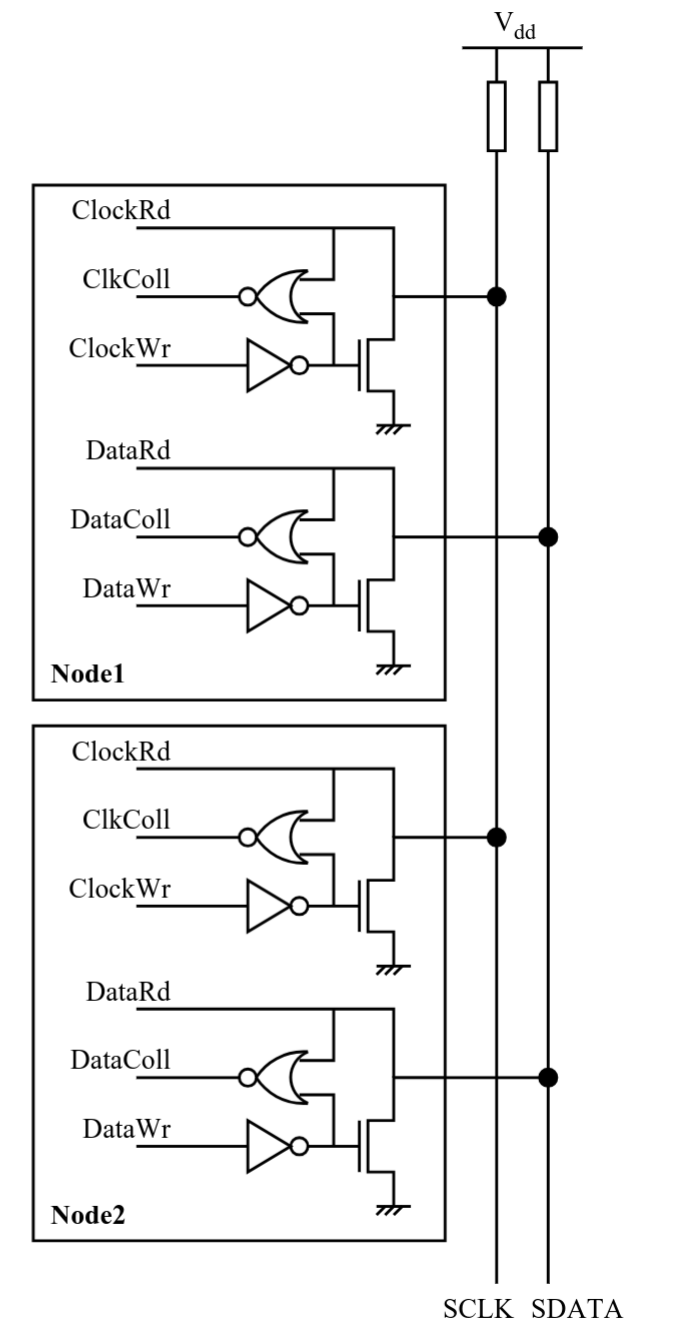
\includegraphics[scale=0.22]{../figures/i2c_pulls.png}
\end{center}

This means that when I2C is idle, both lines are normally high.

\par\smallskip

The architecture allows for detecting collisions on SCLK and SDATA.

A collision happens when a node generates 0, another generates 1.
\begin{itemize}
\item	The output nMOS transistor of the node generating 0 is ON.
\item The output nMOS transistor of the node generating 1 is OFF.
\end{itemize}
There is no short circuit, no damages to the system, and the line just goes to 0 (the nMOS outputting 0 wins).

All nodes constantly monitor the SCLK and SDATA lines:
\begin{itemize}
	\item The device generating the 1 detects the collision;
	\item The device generating the 0 does not notice.
\end{itemize}

\par\smallskip

Two kinds of collisions, actually features:
\begin{itemize}
	\item On the SCLK line we have \textit{clock stretching};
	\item On the SDATA line we have \textit{arbitration}.
\end{itemize}

\subsubsection{I2C addressing}

Each slave in an I2C network is assigned a unique \textbf{address} on 7 bits. This means we have a maximum of 128 slaves, but typically much less.
Nonetheless, there exists a protocol extension to 10-bit addresses.

Some addresses are reserved, and masters do not need an address.

The address is often hardwired in a slave by connecting pins to $V_{dd}$ or ground.
Some bits are not configurable (usually the MSBs) to save on the number of pins on the slave.
The master sends the address of the target slave at the beginning of a transmission, to address it.

\subsubsection{I2C protocol}

SCLK and SDATA lines are normally high when there is no transmission: this just means that all low side nMOS output transistors are OFF.

The main rule is that the SDATA line is allowed to change only when SCLK is low.
Two exceptions mark frames:
\begin{itemize}
	\item \textbf{START} configuration: SDATA makes a high to low transition while SCLK is high;
	\item \textbf{STOP} configuration: SDATA make a low to high transition while SCLK is high.
\end{itemize}

Now:
\begin{enumerate}
	\item All communications begin with a START configuration;
\begin{center}
	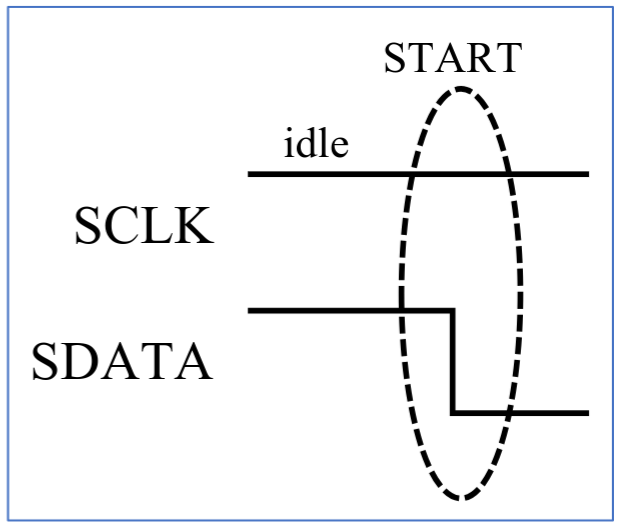
\includegraphics[scale=0.22]{../figures/i2c_form_start.png}
\end{center}

	\item An addressing phase follows: the master activates the clock and generates on SDATA the target slave address on 7 bits, MSB first, one bit per clock cycle.
		
		One more bit is needed for the R/W flag (R when high).
		Then we get one low bit from the slave before releasing the SDATA line (the ACK).

SDATA usually changes only when SCLK is low, shortly after the falling edge of SCLK.
Slaves samples SDATA immediately after the rising edge of SCLK.

\begin{center}
	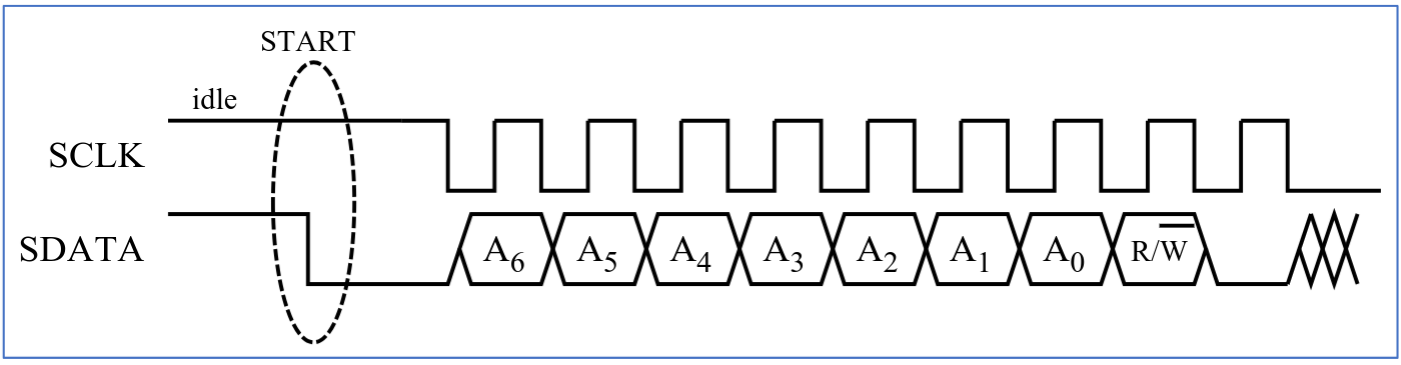
\includegraphics[scale=0.22]{../figures/i2c_form_addr.png}
\end{center}

	\item A data exchange phase in a single direction is next.
We said that the master generates 9 clock cycles: 8 bits for data, 1 bit for ACK.

Now the situation changes depending on the type of operation the master initiates:
\begin{itemize}
	\item \textit{Write}:
\begin{itemize}
\item The master regains control of SDATA and generates 8 data bits, MSB first;
\item The slave generates ACK on the last bit (SDATA=0).
\end{itemize}
	\item \textit{Read}:
\begin{itemize}
\item The slave keeps control of SDATA and generates 8 data bits, MSB first;
\item The master generates ACK on the last bit (SDATA=0).
\end{itemize}
\end{itemize}

This way, only a byte is transferred.
Multiple bytes can be transferred one after the other, with no limit;

\begin{center}
	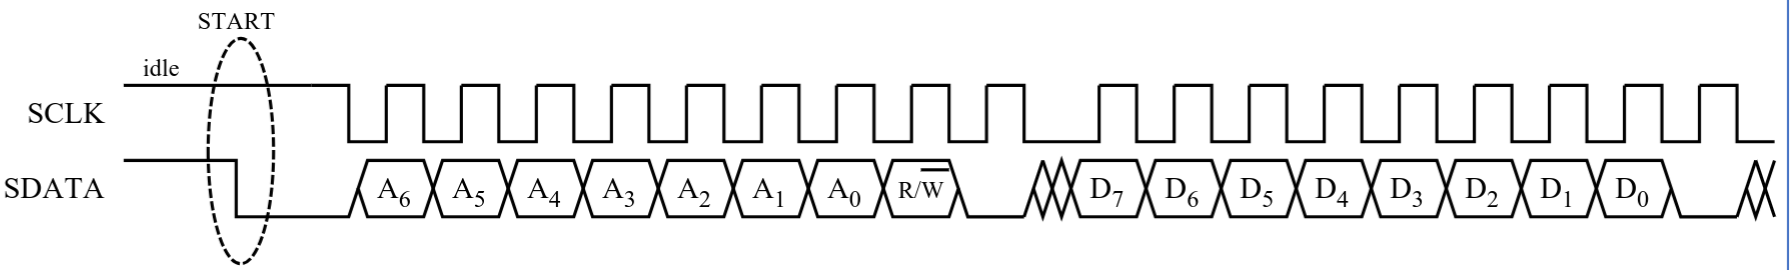
\includegraphics[scale=0.22]{../figures/i2c_form_data.png}
\end{center}

	\item A STOP configuration concludes the communication.

After the last data byte, the master (or the slave, on writes) keeps SDATA low (the ACK).

Then, the master itself keeps SDATA low while releasing the SCLK: SCLK goes high.
When the master then releases SDATA as well, SDATA makes a low to high transition, which signals the STOP configuration.

\begin{center}
	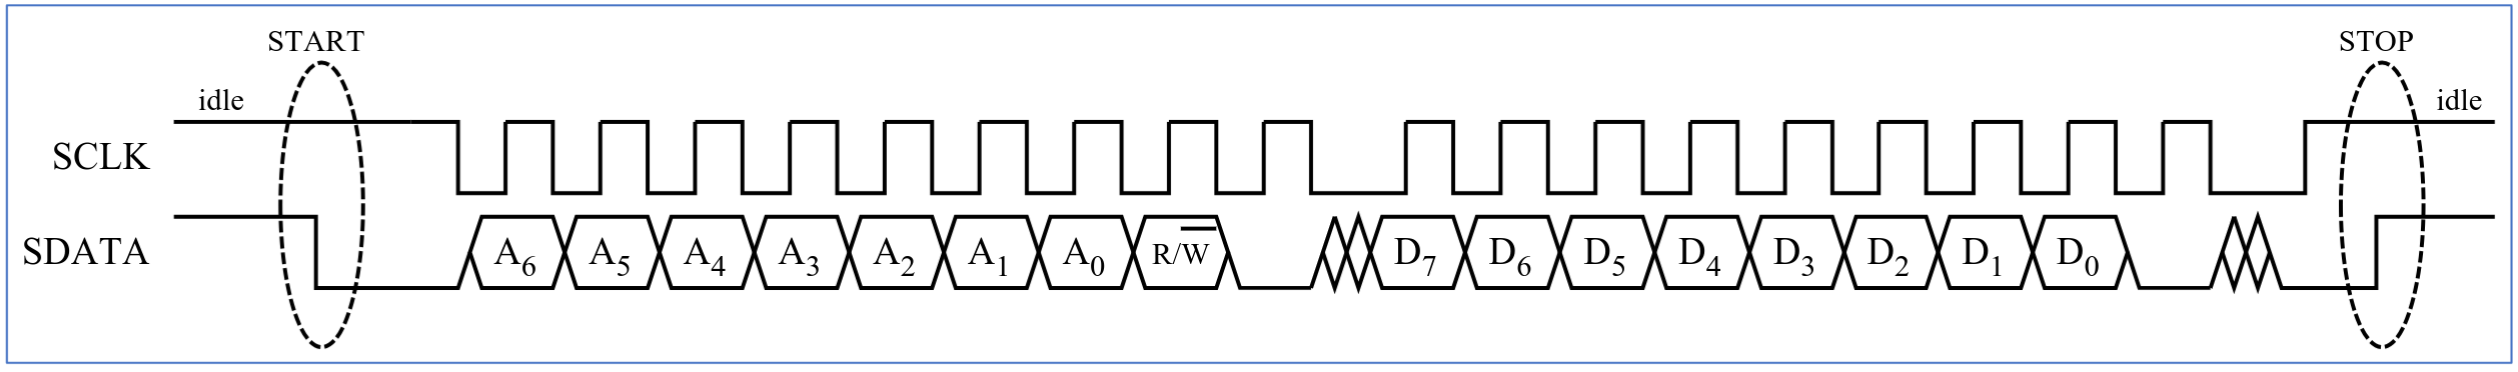
\includegraphics[scale=0.17]{../figures/i2c_form_full.png}
\end{center}

The bus is now idle again. Hooray.
\end{enumerate}

Lastly, let's note the difference between a read and a write operation performed by the master:
\begin{center}
	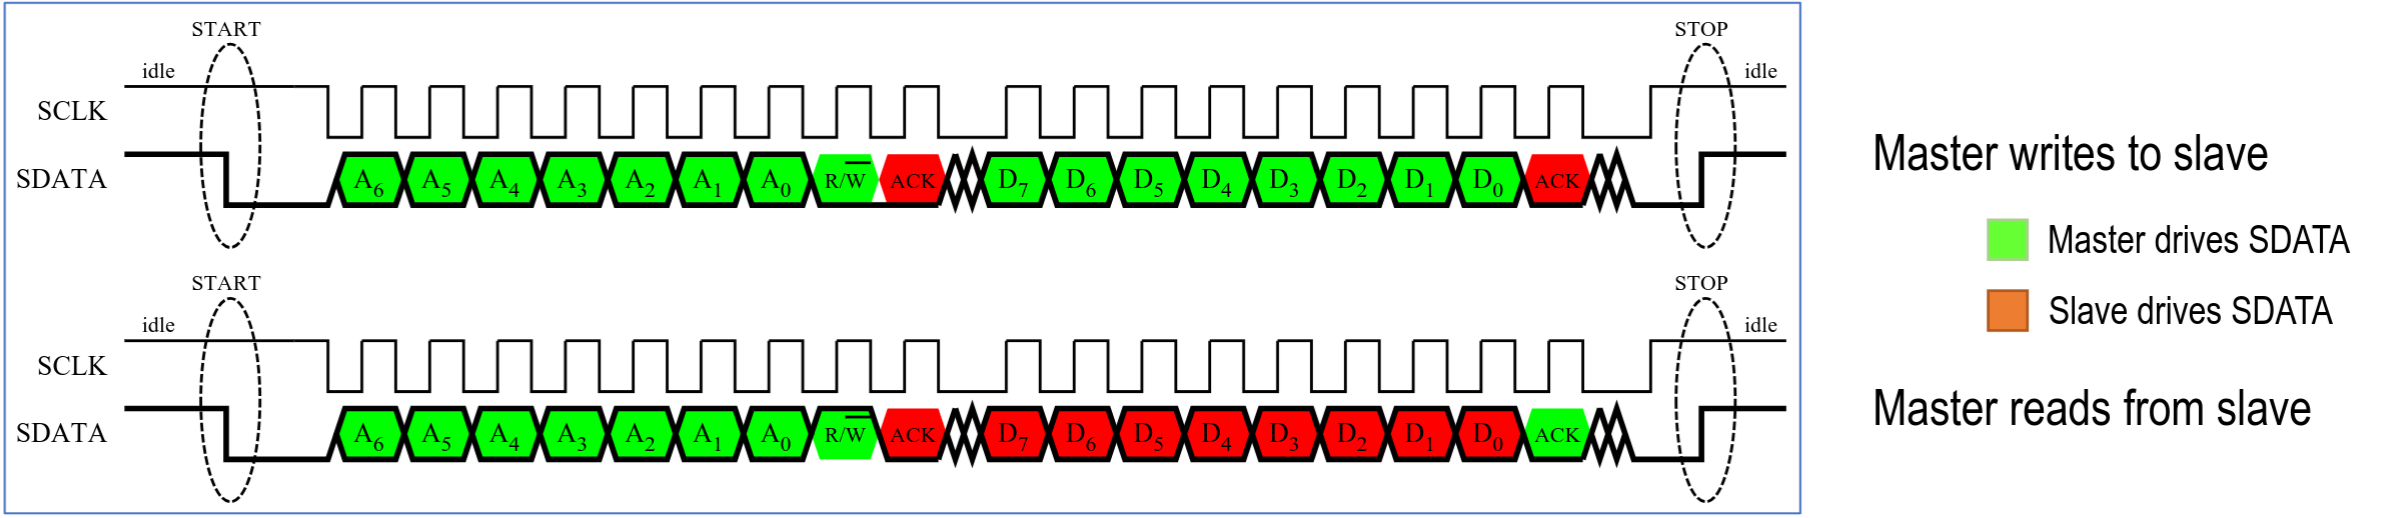
\includegraphics[scale=0.19]{../figures/i2c_form_diff.png}
\end{center}

Some other rules:
\begin{itemize}
\item The first 8 bits are driven by the transmitter (TX), always a master for the addressing phase, a master or a slave in the data phase;
\item The ACK bit is driven by the receiver (RX), always a slave for the addressing phase, a master or a slave in the data phase;
\item Before and after ACK the SDATA line may show oscillations while control passes from TX to RX and viceversa. Oscillations only happen while SCLK is low, and SDATA must become stable before the rising edge of SCLK;
\item An ACK after the addressing phase means the slave is ready for transmission.
	If the ACK is missing (i.e. SDATA=1), the transmission is immediately aborted;
\item An ACK after the data phase, writing to slave means the slave received the data.
It doesn’t mean it was received correctly, as there is no error detection on bits.
If the ACK is missing, the data definitely was not received correctly;
\item An ACK after the data phase, reading from slave means the master is ready to receive an additional byte.
If the ACK is missing, no more bytes are requested by the master.
\end{itemize}

The opposite of an ACK (leaving the SDATA rail up) is called a NACK.

\par\smallskip

A \textbf{RESET} configuration is needed as sometimes a master needs to write a command to a slave, and then immediately read an answer.

This normally requires two transmissions, the first in writing, the second in reading. If the master doesn’t want other masters to gain control of the bus before the second (reading) transmission, at the end of the first (writing) transmission, it can:
\begin{itemize}
	\item Not generate a STOP configuration;
	\item Generate a START configuration, again.
\end{itemize}

This means that the master sets SDATA high, releases SCLK, sets SDATA low, which signals the RESTART configuration.
The bus never becomes idle, thus no other master can gain control.

\subsubsection{Clock stretching}

Let's have a look at the first case in which we use collision detection.
We focus on collision detection on the SCLOCK line, that is \textbf{clock stretching}.

Normally the clock on SCLK is generated by a master, for all bits: a slave should be sufficiently fast to operate at the clock frequency generated by the master.
In this case, the slave only receives the clock and never writes it.

A slow slave may extend the time at which the clock is low, simply by activating its own nMOS transistor on the SCLK line, while it is already forced low by the master.
When the master releases SCLK, the line remains low: the master detects the collision and waits for the SCLK line to be released by the slave, as well.

The communication then proceeds as usual.

If clock stretching is used, individual bits may have different bit time.
Note that not all masters and slaves support clock stretching.

\subsubsection{Arbitration}

This is the second mechanism in which collision detection is used.
We focus on collision detection on the SDATA line, that is \textbf{arbitration}.

Multiple master may wish to start a transmission at the same time.
If the bus is busy, a master shall not start a transmission.
If two masters Master1 and Master2 (or more) concurrently generate a START configuration, they won’t notice it, as they are both driving the same line low: each master believes he is the only owner of the bus!

We assume in the following time that they generate the same clock, and during the addressing phase, they (probably) generate two different addresses.
If at a certain bit Master1 generates a 0 and Master2 generates a 1, that address line goes low: Master1 does not notice any problem, Master2 detects a collision on SDATA.
At this point Master2 has lost the contention and stops the transmission, so that Master1 can complete the transmission.

\end{document}
